\subsection{Synthetic multi-server catalogs (MCP-02)}
\paragraph{Index depth.} At 1024 resources the layout sweep (Table~\ref{tab:mcp02-pilot_gpu-layout},
Figure~\ref{fig:layout}) separates three regimes:
\begin{itemize}
\item paging a flat root or a single server facet exhausts the 40-call budget even for the oracle;
\item two facets are not enough either;
\item three or four facets (server, collection and name bucket, or kind, bucket and entity) let the oracle finish in
14 to 20 calls while reading about half the tool-result bytes of a shallow walk.
\end{itemize}
Deeper indices therefore pay for their traversal once the catalog no longer fits a few pages per node.
Certified exclusions cost refine calls but prune whole provenance or capability subtrees. With the provenance
facet first they remove archive and replica branches in one step, and no certified exclusion ever removed a
required record.

\paragraph{Controls.} Search and eager flat listing are easy for BM25 and the deterministic rules at both catalog
sizes. Layered discovery without search is hard: at 1024 resources both controls solve only a few episodes per cell,
while the oracle solves nearly all of them. That gap is where learned routing can matter.

\paragraph{Learned routers.} Tables~\ref{tab:mcp02-pilot_cpu-success} and \ref{tab:mcp02-pilot_gpu-success} give
accepted episodes per cell for the CPU pilot (width 48, tokens-only encoder) and the GPU pilot (width 128, exact-match
channel). The encoder dominates. Tokens-only routers stay below BM25 in most cells, because they never learn to
recognise that a candidate's identifier equals the needed one. Adding the exact-match channel lifts held-out dev
ranking accuracy from 0.73 to 0.91 for the same Transformer-L2 and data, and it is what lets learned routers compete.
Among tokens-only routers the TRM is the strongest learned family in the layered arms, consistent with recurrence
helping when matching must be learned.

\IfFileExists{tables/mcp02_pilot_gpu_success.tex}{\begin{table}[t]
\centering
\small
\begin{adjustbox}{max width=\linewidth}
\begin{tabular}{lcccccccccc}
\toprule
Router & flat@256 & layered/KBE@256 & layered/SCB@256 & layered\_ldt/PSCB@256 & search@256 & flat@1024 & layered/KBE@1024 & layered/SCB@1024 & layered\_ldt/PSCB@1024 & search@1024 \\
\midrule
dense\_d128 & 32/32 & 28/32 & 24/32 & 22/32 & 32/32 & 32/32 & 7/32 & 5/32 & 5/32 & 32/32 \\
deterministic\_rules & 32/32 & 22/32 & 12/32 & 10/32 & 32/32 & 32/32 & 2/32 & 5/32 & 3/32 & 32/32 \\
hrm\_h2l1\_d128 & 32/32 & 30/32 & 30/32 & 27/32 & 32/32 & 32/32 & 17/32 & 10/32 & 5/32 & 31/32 \\
lexical\_bm25 & 32/32 & 22/32 & 11/32 & 7/32 & 32/32 & 32/32 & 6/32 & 1/32 & 1/32 & 32/32 \\
looped\_p12\_d128 & 32/32 & 31/32 & 28/32 & 27/32 & 32/32 & 32/32 & 20/32 & 11/32 & 8/32 & 31/32 \\
looped\_p4\_d128 & 32/32 & 32/32 & 29/32 & 27/32 & 32/32 & 32/32 & 18/32 & 13/32 & 10/32 & 31/32 \\
oracle\_upper\_bound & 32/32 & 32/32 & 32/32 & 32/32 & 32/32 & 32/32 & 26/32 & 31/32 & 31/32 & 32/32 \\
sham\_random & 10/32 & 0/32 & 1/32 & 0/32 & 27/32 & 8/32 & 0/32 & 0/32 & 0/32 & 21/32 \\
sham\_shuffled\_transformer\_l2\_d128 & 0/32 & 0/32 & 0/32 & 0/32 & 11/32 & 0/32 & 0/32 & 0/32 & 0/32 & 11/32 \\
transformer\_l1\_d128 & 32/32 & 29/32 & 30/32 & 26/32 & 32/32 & 32/32 & 19/32 & 10/32 & 7/32 & 31/32 \\
transformer\_l2\_d128 & 32/32 & 32/32 & 28/32 & 25/32 & 32/32 & 32/32 & 22/32 & 9/32 & 6/32 & 31/32 \\
transformer\_l2\_d128\_tokens & 26/32 & 24/32 & 16/32 & 8/32 & 32/32 & 20/32 & 9/32 & 1/32 & 0/32 & 27/32 \\
transformer\_l4\_d128 & 32/32 & 31/32 & 30/32 & 27/32 & 32/32 & 32/32 & 23/32 & 14/32 & 9/32 & 31/32 \\
trm\_c2i1\_d128 & 32/32 & 30/32 & 31/32 & 28/32 & 32/32 & 32/32 & 15/32 & 10/32 & 5/32 & 31/32 \\
trm\_c4i2\_d128 & 32/32 & 30/32 & 30/32 & 26/32 & 32/32 & 32/32 & 14/32 & 9/32 & 4/32 & 31/32 \\
trm\_ldt\_c2i1\_d128 & 32/32 & 32/32 & 32/32 & 27/32 & 32/32 & 32/32 & 20/32 & 8/32 & 6/32 & 31/32 \\
\bottomrule
\end{tabular}
\end{adjustbox}
\caption{MCP-02 pilot gpu: accepted episodes per arm and catalog size (32 held-out test worlds per cell, 40-call budget).}
\label{tab:mcp02-pilot_gpu-success}
\end{table}
}{}
\IfFileExists{tables/mcp02_pilot_cpu_success.tex}{\begin{table}[t]
\centering
\small
\begin{adjustbox}{max width=\linewidth}
\begin{tabular}{lcccccccccc}
\toprule
Router & flat@256 & layered/KBE@256 & layered/SCB@256 & layered\_ldt/PSCB@256 & search@256 & flat@1024 & layered/KBE@1024 & layered/SCB@1024 & layered\_ldt/PSCB@1024 & search@1024 \\
\midrule
dense\_d48 & 17/32 & 1/32 & 1/32 & 2/32 & 30/32 & 11/32 & 0/32 & 0/32 & 0/32 & 29/32 \\
deterministic\_rules & 32/32 & 22/32 & 12/32 & 10/32 & 32/32 & 32/32 & 2/32 & 5/32 & 3/32 & 32/32 \\
hrm\_h2l1\_d48 & 18/32 & 16/32 & 6/32 & 3/32 & 28/32 & 9/32 & 6/32 & 0/32 & 0/32 & 20/32 \\
lexical\_bm25 & 32/32 & 22/32 & 11/32 & 7/32 & 32/32 & 32/32 & 6/32 & 1/32 & 1/32 & 32/32 \\
looped\_p4\_d48 & 16/32 & 11/32 & 5/32 & 4/32 & 30/32 & 13/32 & 8/32 & 0/32 & 0/32 & 24/32 \\
oracle\_upper\_bound & 32/32 & 32/32 & 32/32 & 32/32 & 32/32 & 32/32 & 26/32 & 31/32 & 31/32 & 32/32 \\
sham\_random & 10/32 & 0/32 & 1/32 & 0/32 & 27/32 & 8/32 & 0/32 & 0/32 & 0/32 & 21/32 \\
sham\_shuffled\_transformer\_l2\_d48 & 1/32 & 1/32 & 0/32 & 0/32 & 21/32 & 2/32 & 0/32 & 0/32 & 0/32 & 21/32 \\
transformer\_l1\_d48 & 16/32 & 13/32 & 4/32 & 3/32 & 28/32 & 7/32 & 3/32 & 0/32 & 0/32 & 21/32 \\
transformer\_l2\_d48 & 16/32 & 17/32 & 4/32 & 5/32 & 30/32 & 8/32 & 5/32 & 1/32 & 0/32 & 19/32 \\
transformer\_l2\_d48\_match & 32/32 & 31/32 & 29/32 & 26/32 & 32/32 & 32/32 & 16/32 & 9/32 & 6/32 & 31/32 \\
transformer\_l4\_d48 & 19/32 & 17/32 & 6/32 & 4/32 & 26/32 & 12/32 & 8/32 & 0/32 & 0/32 & 26/32 \\
trm\_c2i1\_d48 & 18/32 & 20/32 & 7/32 & 5/32 & 27/32 & 10/32 & 2/32 & 0/32 & 0/32 & 23/32 \\
trm\_c2i1\_d48\_match & 32/32 & 30/32 & 29/32 & 28/32 & 32/32 & 32/32 & 20/32 & 12/32 & 3/32 & 28/32 \\
trm\_ldt\_c2i1\_d48 & 18/32 & 17/32 & 5/32 & 3/32 & 31/32 & 10/32 & 1/32 & 0/32 & 0/32 & 21/32 \\
\bottomrule
\end{tabular}
\end{adjustbox}
\caption{MCP-02 pilot cpu: accepted episodes per arm and catalog size (32 held-out test worlds per cell, 40-call budget).}
\label{tab:mcp02-pilot_cpu-success}
\end{table}
}{}
\IfFileExists{tables/mcp02_pilot_gpu_depth.tex}{\begin{table}[t]
\centering
\small
\begin{adjustbox}{max width=\linewidth}
\begin{tabular}{lrrrrr}
\toprule
Router & Arm & Test depth & Accepted & Calls/ep & GFLOPs/ep \\
\midrule
hrm\_h2l1\_d128 & layered/SCB & 1 & 30/32 & 18.28 & 26.06 \\
hrm\_h2l1\_d128 & layered/SCB & 2 & 30/32 & 18.34 & 52.32 \\
hrm\_h2l1\_d128 & layered/SCB & 4 & 30/32 & 18.47 & 105.19 \\
hrm\_h2l1\_d128 & layered/SCB & 8 & 30/32 & 18.41 & 209.26 \\
hrm\_h2l1\_d128 & layered\_ldt/PSCB & 1 & 25/32 & 26.62 & 29.94 \\
hrm\_h2l1\_d128 & layered\_ldt/PSCB & 2 & 27/32 & 25.12 & 56.33 \\
hrm\_h2l1\_d128 & layered\_ldt/PSCB & 4 & 27/32 & 25.41 & 115.21 \\
hrm\_h2l1\_d128 & layered\_ldt/PSCB & 8 & 27/32 & 25.56 & 232.96 \\
looped\_p4\_d128 & layered/SCB & 1 & 25/32 & 25.31 & 20.32 \\
looped\_p4\_d128 & layered/SCB & 2 & 27/32 & 22.84 & 36.25 \\
looped\_p4\_d128 & layered/SCB & 4 & 29/32 & 19.06 & 54.79 \\
looped\_p4\_d128 & layered/SCB & 8 & 30/32 & 18.31 & 101.94 \\
looped\_p4\_d128 & layered\_ldt/PSCB & 1 & 19/32 & 31.72 & 20.35 \\
looped\_p4\_d128 & layered\_ldt/PSCB & 2 & 25/32 & 28.75 & 37.83 \\
looped\_p4\_d128 & layered\_ldt/PSCB & 4 & 27/32 & 24.84 & 55.22 \\
looped\_p4\_d128 & layered\_ldt/PSCB & 8 & 28/32 & 25.44 & 106.32 \\
trm\_c2i1\_d128 & layered/SCB & 1 & 31/32 & 18.19 & 25.50 \\
trm\_c2i1\_d128 & layered/SCB & 2 & 31/32 & 18.47 & 52.14 \\
trm\_c2i1\_d128 & layered/SCB & 4 & 31/32 & 17.81 & 99.10 \\
trm\_c2i1\_d128 & layered/SCB & 8 & 31/32 & 17.81 & 198.08 \\
trm\_c2i1\_d128 & layered\_ldt/PSCB & 1 & 27/32 & 25.72 & 28.09 \\
trm\_c2i1\_d128 & layered\_ldt/PSCB & 2 & 28/32 & 25.34 & 53.95 \\
trm\_c2i1\_d128 & layered\_ldt/PSCB & 4 & 28/32 & 25.34 & 108.52 \\
trm\_c2i1\_d128 & layered\_ldt/PSCB & 8 & 28/32 & 25.25 & 215.54 \\
trm\_ldt\_c2i1\_d128 & layered/SCB & 1 & 31/32 & 17.94 & 24.88 \\
trm\_ldt\_c2i1\_d128 & layered/SCB & 2 & 32/32 & 16.88 & 45.53 \\
trm\_ldt\_c2i1\_d128 & layered/SCB & 4 & 32/32 & 16.81 & 90.47 \\
trm\_ldt\_c2i1\_d128 & layered/SCB & 8 & 32/32 & 16.84 & 181.47 \\
trm\_ldt\_c2i1\_d128 & layered\_ldt/PSCB & 1 & 27/32 & 26.56 & 32.32 \\
trm\_ldt\_c2i1\_d128 & layered\_ldt/PSCB & 2 & 27/32 & 25.59 & 61.92 \\
trm\_ldt\_c2i1\_d128 & layered\_ldt/PSCB & 4 & 28/32 & 24.75 & 119.49 \\
trm\_ldt\_c2i1\_d128 & layered\_ldt/PSCB & 8 & 28/32 & 24.69 & 240.16 \\
\bottomrule
\end{tabular}
\end{adjustbox}
\caption{Recurrent depth changed at test time only (trained depth in the router name).}
\label{tab:mcp02-pilot_gpu-depth}
\end{table}
}{}
\IfFileExists{tables/mcp02_pilot_gpu_layout.tex}{\begin{table}[t]
\centering
\small
\begin{adjustbox}{max width=\linewidth}
\begin{tabular}{lrrrrrrr}
\toprule
Router & Arm & Layout & Depth & Accepted & Calls/ep & Result KB/ep & Certified excl. \\
\midrule
deterministic\_rules & layered & - & 1 & 0/16 & 40.00 & 82.60 & 0 \\
deterministic\_rules & layered & S & 2 & 0/16 & 40.00 & 111.37 & 0 \\
deterministic\_rules & layered & SC & 3 & 0/16 & 40.00 & 79.23 & 0 \\
deterministic\_rules & layered & KBE & 4 & 0/16 & 40.00 & 103.58 & 0 \\
deterministic\_rules & layered & KSB & 4 & 1/16 & 38.06 & 85.82 & 0 \\
deterministic\_rules & layered & SCB & 4 & 3/16 & 34.94 & 81.71 & 0 \\
deterministic\_rules & layered & PKBE & 5 & 1/16 & 38.94 & 94.73 & 0 \\
deterministic\_rules & layered & PSCB & 5 & 1/16 & 38.75 & 130.26 & 0 \\
deterministic\_rules & layered\_ldt & - & 1 & 0/16 & 40.00 & 111.89 & 1292 \\
deterministic\_rules & layered\_ldt & S & 2 & 0/16 & 40.00 & 103.49 & 700 \\
deterministic\_rules & layered\_ldt & SC & 3 & 0/16 & 40.00 & 79.41 & 5 \\
deterministic\_rules & layered\_ldt & KBE & 4 & 5/16 & 38.00 & 92.45 & 85 \\
deterministic\_rules & layered\_ldt & KSB & 4 & 1/16 & 38.25 & 77.62 & 96 \\
deterministic\_rules & layered\_ldt & SCB & 4 & 3/16 & 35.12 & 80.09 & 141 \\
deterministic\_rules & layered\_ldt & PKBE & 5 & 1/16 & 38.81 & 79.05 & 92 \\
deterministic\_rules & layered\_ldt & PSCB & 5 & 1/16 & 38.75 & 103.28 & 92 \\
oracle\_upper\_bound & layered & - & 1 & 0/16 & 40.00 & 83.64 & 0 \\
oracle\_upper\_bound & layered & S & 2 & 1/16 & 39.06 & 103.91 & 0 \\
oracle\_upper\_bound & layered & SC & 3 & 6/16 & 30.44 & 80.67 & 0 \\
oracle\_upper\_bound & layered & KBE & 4 & 14/16 & 16.56 & 38.79 & 0 \\
oracle\_upper\_bound & layered & KSB & 4 & 13/16 & 20.31 & 64.14 & 0 \\
oracle\_upper\_bound & layered & SCB & 4 & 15/16 & 14.06 & 40.86 & 0 \\
oracle\_upper\_bound & layered & PKBE & 5 & 13/16 & 19.50 & 38.60 & 0 \\
oracle\_upper\_bound & layered & PSCB & 5 & 10/16 & 23.94 & 49.16 & 0 \\
oracle\_upper\_bound & layered\_ldt & - & 1 & 0/16 & 40.00 & 116.96 & 1292 \\
oracle\_upper\_bound & layered\_ldt & S & 2 & 1/16 & 39.06 & 109.34 & 467 \\
oracle\_upper\_bound & layered\_ldt & SC & 3 & 5/16 & 31.50 & 82.82 & 48 \\
oracle\_upper\_bound & layered\_ldt & KBE & 4 & 15/16 & 19.19 & 40.13 & 97 \\
oracle\_upper\_bound & layered\_ldt & KSB & 4 & 14/16 & 20.62 & 59.78 & 96 \\
oracle\_upper\_bound & layered\_ldt & SCB & 4 & 15/16 & 15.69 & 44.02 & 7 \\
oracle\_upper\_bound & layered\_ldt & PKBE & 5 & 14/16 & 21.69 & 39.73 & 153 \\
oracle\_upper\_bound & layered\_ldt & PSCB & 5 & 15/16 & 20.56 & 46.15 & 158 \\
trm\_c2i1\_d128 & layered & - & 1 & 0/16 & 40.00 & 84.12 & 0 \\
trm\_c2i1\_d128 & layered & S & 2 & 1/16 & 39.06 & 128.38 & 0 \\
trm\_c2i1\_d128 & layered & SC & 3 & 1/16 & 38.50 & 130.15 & 0 \\
trm\_c2i1\_d128 & layered & KBE & 4 & 8/16 & 34.56 & 76.22 & 0 \\
trm\_c2i1\_d128 & layered & KSB & 4 & 7/16 & 34.12 & 128.74 & 0 \\
trm\_c2i1\_d128 & layered & SCB & 4 & 6/16 & 33.75 & 107.08 & 0 \\
trm\_c2i1\_d128 & layered & PKBE & 5 & 4/16 & 35.12 & 72.11 & 0 \\
trm\_c2i1\_d128 & layered & PSCB & 5 & 2/16 & 36.75 & 106.22 & 0 \\
trm\_c2i1\_d128 & layered\_ldt & - & 1 & 0/16 & 40.00 & 116.95 & 1292 \\
trm\_c2i1\_d128 & layered\_ldt & S & 2 & 1/16 & 39.06 & 112.60 & 565 \\
trm\_c2i1\_d128 & layered\_ldt & SC & 3 & 1/16 & 38.56 & 138.73 & 526 \\
trm\_c2i1\_d128 & layered\_ldt & KBE & 4 & 6/16 & 35.31 & 76.15 & 88 \\
trm\_c2i1\_d128 & layered\_ldt & KSB & 4 & 7/16 & 35.25 & 127.07 & 93 \\
trm\_c2i1\_d128 & layered\_ldt & SCB & 4 & 6/16 & 34.12 & 105.65 & 102 \\
trm\_c2i1\_d128 & layered\_ldt & PKBE & 5 & 5/16 & 36.25 & 70.03 & 122 \\
trm\_c2i1\_d128 & layered\_ldt & PSCB & 5 & 3/16 & 37.06 & 105.20 & 115 \\
trm\_ldt\_c2i1\_d128 & layered & - & 1 & 0/16 & 40.00 & 84.13 & 0 \\
trm\_ldt\_c2i1\_d128 & layered & S & 2 & 0/16 & 40.00 & 145.81 & 0 \\
trm\_ldt\_c2i1\_d128 & layered & SC & 3 & 2/16 & 36.62 & 124.36 & 0 \\
trm\_ldt\_c2i1\_d128 & layered & KBE & 4 & 10/16 & 33.00 & 73.03 & 0 \\
trm\_ldt\_c2i1\_d128 & layered & KSB & 4 & 5/16 & 35.19 & 135.66 & 0 \\
trm\_ldt\_c2i1\_d128 & layered & SCB & 4 & 5/16 & 32.62 & 110.71 & 0 \\
trm\_ldt\_c2i1\_d128 & layered & PKBE & 5 & 4/16 & 36.81 & 74.51 & 0 \\
trm\_ldt\_c2i1\_d128 & layered & PSCB & 5 & 4/16 & 34.00 & 97.48 & 0 \\
trm\_ldt\_c2i1\_d128 & layered\_ldt & - & 1 & 0/16 & 40.00 & 90.18 & 243 \\
trm\_ldt\_c2i1\_d128 & layered\_ldt & S & 2 & 0/16 & 40.00 & 132.92 & 208 \\
trm\_ldt\_c2i1\_d128 & layered\_ldt & SC & 3 & 2/16 & 36.81 & 124.50 & 17 \\
trm\_ldt\_c2i1\_d128 & layered\_ldt & KBE & 4 & 4/16 & 36.62 & 67.21 & 54 \\
trm\_ldt\_c2i1\_d128 & layered\_ldt & KSB & 4 & 4/16 & 35.50 & 134.13 & 59 \\
trm\_ldt\_c2i1\_d128 & layered\_ldt & SCB & 4 & 6/16 & 32.94 & 110.87 & 4 \\
trm\_ldt\_c2i1\_d128 & layered\_ldt & PKBE & 5 & 1/16 & 39.00 & 62.86 & 98 \\
trm\_ldt\_c2i1\_d128 & layered\_ldt & PSCB & 5 & 4/16 & 35.31 & 99.94 & 122 \\
\bottomrule
\end{tabular}
\end{adjustbox}
\caption{Index layout and depth at 1024 resources: deeper facet hierarchies against traversal cost.}
\label{tab:mcp02-pilot_gpu-layout}
\end{table}
}{}
\IfFileExists{figures/mcp02_layout_depth.pdf}{
\begin{figure}[t]\centering
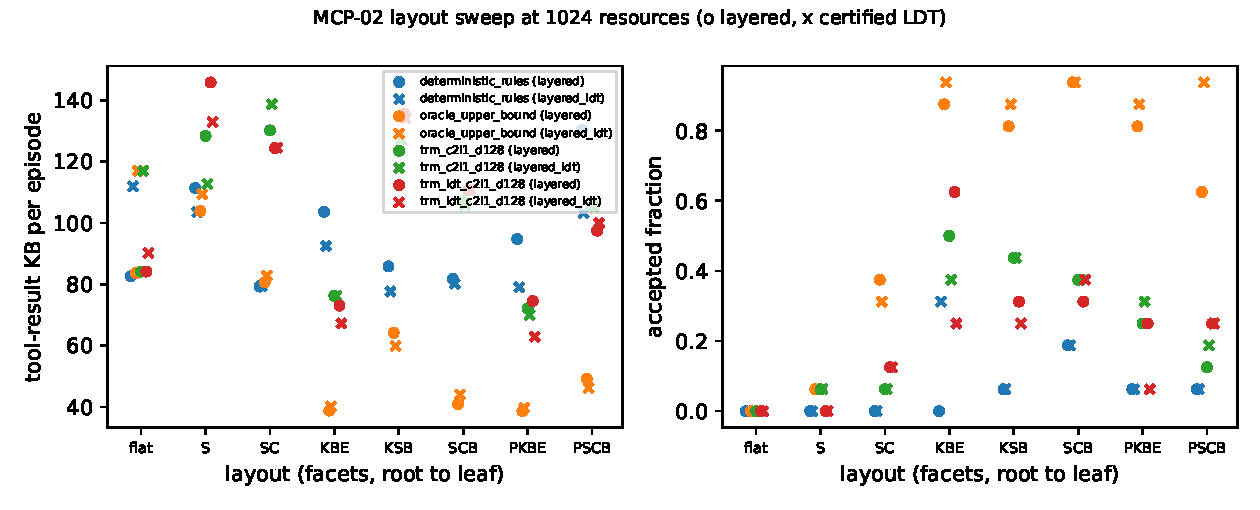
\includegraphics[width=0.95\linewidth]{figures/mcp02_layout_depth.pdf}
\caption{MCP-02 index depth against tool-result volume and accepted episodes (1024 resources).}\label{fig:layout}
\end{figure}}{}
